\section{План тестирования} \label{sub26}

\textbf{Тест~1.}

\textbf{Цель.} 

Проверить отсутствие подсветки полей, которые не~являются членами скрипта метаданных.

\textbf{Порядок выполнения.} 

\begin{enumerate} 
\item{Оставить скрипт метаданных пустым.}
\item{Ввести название любой переменной в~скрипте сценария исполнения, не~определённой в~контексте данного скрипта.}
\item{Убедиться, что редактор сообщил об~ошибке.}
\end{enumerate}

\textbf{Результат.} 

Успешное выполнение теста представлено на~рис.~\ref{img:test-1}.

\begin{figure}[h!]
	\centering
	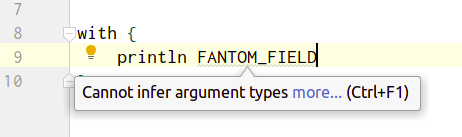
\includegraphics [scale=0.7] {test1}
	\caption{Пример отсутствия подсветки у~поля, не~определённого в~скрипте метаданных}
	\label{img:test-1}
\end{figure}

В~случае не~прохождения теста редактор не~сообщит об~ошибке.

\textbf{Тест 2.}

\textbf{Цель.} 

Проверить подсветку поля, которое определенно в~скрипте метаданных.

\textbf{Порядок выполнения.} 

\begin{enumerate} 
	\item{Определить поле \texttt{TEST\_FIELD} типа \texttt{String} в~скрипте метаданных.}
	\item{Ввести название переменную \texttt{TEST\_FIELD} в~скрипте сценария исполнения.}
	\item{Убедиться, что редактор подсветил переменную.}
\end{enumerate}

\textbf{Результат.} 

Успешное выполнение теста представлено на~рис.~\ref{img:test-2}.

\begin{figure}[h!]
	\centering
	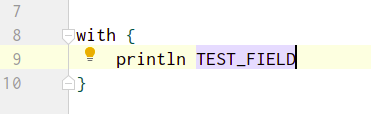
\includegraphics [scale=0.7] {test2}
	\caption{Пример подсветки поля, определённого в~скрипте метаданных}
	\label{img:test-2}
\end{figure}

В~случае не~прохождения теста редактор не~подсветит переменную.

\textbf{Тест 3.}

\textbf{Цель.} 

Проверить авто-дополнения имени поля во~время набора текста.

\textbf{Порядок выполнения.} 

\begin{enumerate} 
	\item{Определить поле \texttt{TEST\_FIELD} типа \texttt{String} в~скрипте метаданных.}
	\item{Начать вводить название переменной \texttt{TEST\_FIELD} в~скрипте сценария исполнения.}
	\item{Убедиться, что редактор предлагает авто-дополнение к~имени переменной.}
\end{enumerate}

\textbf{Результат.} 

Успешное выполнение теста представлено на~рис.~\ref{img:test-3}.

\begin{figure}[h!]
	\centering
	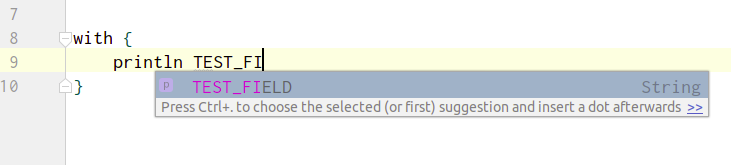
\includegraphics [scale=0.65] {test3}
	\caption{Пример авто-дополнения поля, определённого в~скрипте метаданных}
	\label{img:test-3}
\end{figure}

В~случае не~прохождения теста редактор не~предложит авто-дополнение.

\textbf{Тест 4.}

\textbf{Цель.} 

Убедиться в~корректной проверки типов.

\textbf{Порядок выполнения.} 

\begin{enumerate} 
	\item{Определить поле \texttt{TEST\_FIELD} типа \texttt{String} в~скрипте метаданных.}
	\item{В~скрипте сценария исполнения написать выражение \\ 
		\texttt{Integer~i~=~TEST\_FIELD~+~1}.}
	\item{Убедиться, что редактор сообщает о~некорректности данного выражения из-за несоответствия типов.}
\end{enumerate}

\textbf{Результат.} 

Успешное выполнение теста представлено на~рис.~\ref{img:test-4}.

\begin{figure}[h!]
	\centering
	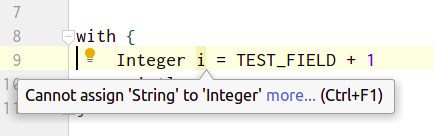
\includegraphics [scale=0.7] {test4}
	\caption{Пример определения типа у~поля, определённого в~скрипте метаданных}
	\label{img:test-4}
\end{figure}

В~случае не~прохождения теста редактор идентифицирует выражение корректным, либо сообщение об~ошибке не~будет касаться типов.
